%\setcounter{chapter}{0}
\chapter*{Outline}
\chaptermark{Outline}
\addcontentsline{toc}{chapter}{Outline}

Tell the world what you will do to fill some space in this template!

\setcounter{chapter}{0}
\chapter{Cosmic Rays Test Chapter}
\label{chapter:Approach}
The Text!

Hillas equation: \cite{Hillas}
\begin{equation}
 \left(\frac{B}{\mu G}\right)\left(\frac {R}{kpc}\right) = 2\left(\frac{E}{10^{18}eV}\right)\frac1{Z\beta}
\label{eq:Hillas}
\end{equation}

\begin{figure}
  \centering
  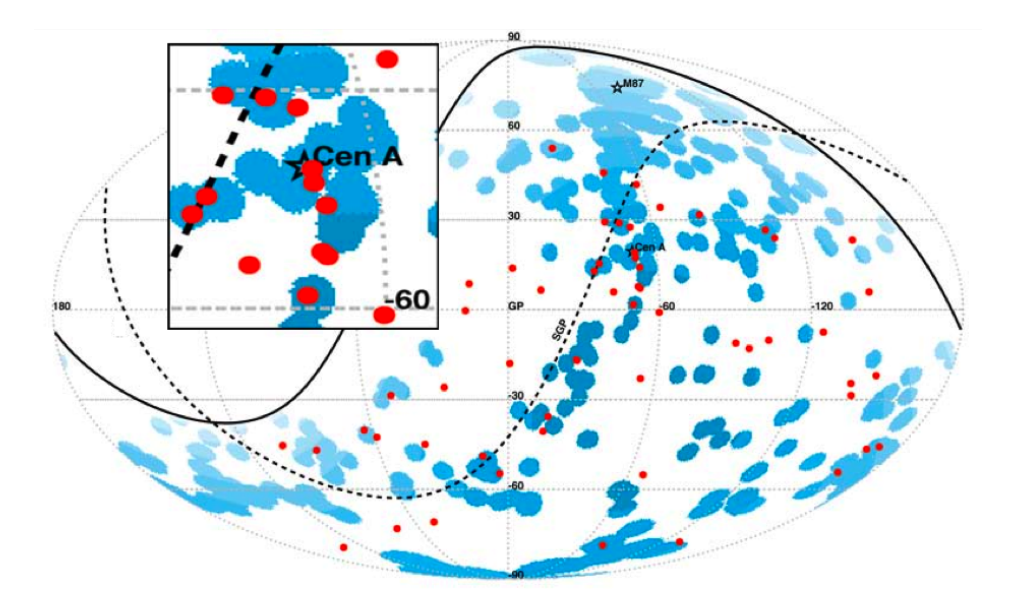
\includegraphics[width=0.9\textwidth]{bilder/AugerAGNplotICRC2009.png}
  \caption[Distribution of events of the highest energies of the Pierre Auger Observatory]{The figure shows an Aitoff projection of the celestial sphere in galactic coordinates. The red dots indicate events above 55 EeV that have been measured with the Pierre Auger Observatory. The blue areas are possible sources from the VCV catalogue. The strength of the blue colour is drawn according to the exposure of the detector. Taken from \cite{Hague2009} }
  \label{fig:AGN}
\end{figure}



